\documentclass[12pt]{article}
%Gummi|065|=)
\title{\textbf{Circuitos de activacion con tiristores CA-CD,CA-CA.}}
\author{Guzman Vazquez Jaime Alan Yamil}
\date{septiembre 24}
\usepackage{graphicx}
\begin{document}

\maketitle

\section{Fundamentos de la tecnologia.}

La tecnologia propuesta considera que cada rectificador tiristorizado se caracteriza por dos  rectificadores basicos , los cuales estan conectados en serie o en paralelo.\\
Los voltajes de salida  de cada rectificador basico estan simetricamnete desplazados  en el tiempo y tiene un periodo "T".\\
tambien se utilizan dos interruptores de conmutacion forzada los cuales estan en serie con los rectificadores basicos y son capaces de darle forma a las corrientesa travez de acciones sucesivas de apertura y cierre  .\\
Esto hace referencia a que los tiristores tienen la funcion no solo de que rectifican las ondas,si no tambien que tienen la capacidad de generar un retraso en ella que puede ser controlado por medio de ecuaciones esto puede ser muy util cuando por ejemplo solo quieres utilizar la mitad de tu onda.  
\begin{figure}[htp]
\centering
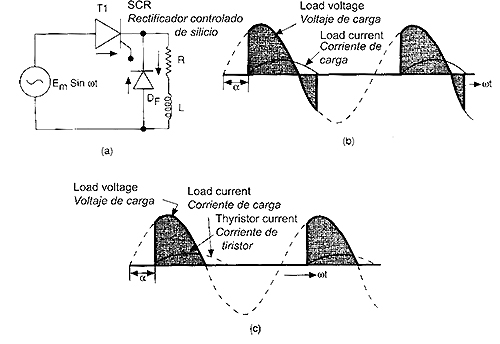
\includegraphics[scale=0.50]{ac_dc.jpg}
\caption{Aqui se muestra el tipo de onda que genera el tiristor.}
\label{}
\end{figure}
\begin{figure}[htp]
\centering
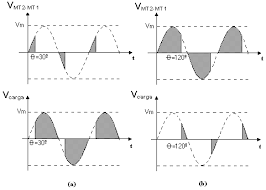
\includegraphics[scale=1]{onda ac-ac.png}
\caption{se puede observar el cambio que realiza el tiristor.}
\label{}
\end{figure}


\maketitle
\section{convertidores AC-DC.}
 Los convertidores de corriente  se sustituyen por asi decirlo los diodos rectificadores , estos son suplantados por tiristores, estos tiristores actuan de una manera similar a los diodos rectificadores, sin embargo tienen la funcion de poder regular el disparo de la onda senoidal para que esta se retrase y asi se encuetre ya en su mayor voltaje al momento de ser disparada si asi se necesita, este disparo de la onda puede ser controlado por medio de el mismo control del tiristor por medio de calculos, estos tiristores se se activan unicamente cuando la  onda senoidal esta de forma positiva apagandose cuando la onda se encuentra en la parte negativa.\\\\
a continuacion observaremos algunas imagenes de este fenomeno:  


\maketitle
\section{Conversores AC-AC}
Estos  tipos de convertidores utilizan el mismo fundamento que los anteriores plannteados pero en corriente alterna a corriente alterna, estos tipos de conversores en vez de rectificar la onda como los anteriores  dejando solo la onda positiva, estos realizan la funcion del disparo en toda la onda senoidal, dando como  resultado el el aplazamiento total de la onda senoidal, en vez de unicamente partirla y solo dejarla pasar del lado positivo.\\
A continuacion se mostraran algunas imagenes de este fenomeno:\\



\maketitle
\section{Tipos de tiristores.}
A continuacion daremos una breve descripcion de los diferentes tipos de tiristores que existen:\\
*Diodo shockley:\\
Este es un tiristor que contiene dos terminales(anodo y catodo) Esta constituido por cuatro capas de semiconductores que forman una estructura pnpn,
este actua como un interruptor: esta abierto hasta que la tension aplicada adquiere cierto valor, Entonces se cierra y este permite la conduccion hasta que se decrese la tension hasta por debajo del umbral  entonces se abre  de nuevo, A este  umbral se le llama (lH).\\\\
*SCR:
(silicon controler rectifier) son las siglas de este componente, este posee varias similitudes con el diod shockley anteriormente descrito solo con la diferencia de que  este posee tres partes que son anodo,catodo y puerta (gate)
realizando una funcion de interruptor.\\\\
*SCS:
(silicon controled switch)por sus siglas en ingles, este es muy similar al SCR con la diferencia de que este posee dos puertas, una para entrar en conduccion y otra para el corte. Este se suele utilizar en potencias menores a las del SCR.\\\\
*DIAC:
Este componente es un tiristor que permite conducir en ambos sentidos, es un dispositivo que es similar a poner dos diodos shockley de forma opuesta.\\\\
*TRIAC:
Este dispositivo es similar al DIAC pero con una sola puerta, se puede disparar con un impulso de voltaje y no  requiere alcanzar el voltaje (VBO) como el DIAC.\\\\ 

referencias
profesormolina2.webcindario.com
\\issuu.com
\\convertidores CA/CA y CA/DC contiristores-universidad de oviedo.pptx
\end{document}
